\textbf{3.8.9 Strengths and Limitations}

DQN has several advantages for the portfolio trading problem considered
in this study. Experience replay lets the agent reuse previous
transitions collected at different stages of training, while the target
network helps to stabilise the learning process. The network also
provides separate value estimates for each valid action, making it
possible to directly compare the expected value of Buy, Hold, and Sell.

However, DQN also has some limitations. Because the network learns by
directly predicting Q-values, its training can be affected by the scale
of the reward and target values. This differs from the REINFORCE
implementation, where returns are standardised within each episode
before the policy update, reducing sensitivity.

Another limitation is that DQN uses bootstrapping. The target partly
relies on Q-value estimates given by the network rather than observed
rewards. If these estimates are inaccurate, the resulting errors can be
carried into later updates and affect future learning.

These differences make DQN a useful comparison to the policy-gradient
algorithms used in this study rather than using another implementation
of the same learning architecture.

\textbf{3.9 PPO: Proximal Policy Optimisation}

Proximal Policy Optimisation (PPO) is used as the third learning method
in this study to provide a more stable policy-gradient algorithm that
can be compared with REINFORCE.

REINFORCE updates the policy using the returns obtained from sampled
episodes. Although this approach is straightforward, the policy can
change considerably between updates, specifically when the sampled
returns are large, making training unstable.

PPO reduces this problem by limiting how much the policy changes during
each update. It does this by comparing the new policy with the policy
from the training data.

\textbf{3.9.1 Actor-Critic Structure \& Advantage Function}

PPO uses two neural networks: an \textbf{actor} and a \textbf{critic}.

The actor represents the portfolio trading policy:

\[\pi_{\theta}\left( a|s \right),\]

where \(\theta\) represents the parameters of the policy network.

The critic estimates the value of the current state:

\[V_{\phi}(s),\]

where \(\phi\) represents the parameters of the value network.

The actor selects actions, while the critic estimates the expected
future return from a given state. The critic therefore provides a
reference to compare the outcome of a policy's action against.

This lets PPO use an \textbf{advantage} value rather than relying
directly on the return of a full episode, like in REINFORCE.

The advantage at time \(t\) can be represented as

\[A_{t} = G_{t} - V_{\phi}\left( s_{t} \right),\]

The advantage shows whether the selected action performed better or
worse than expected for the current state. A positive advantage means
the outcome was better than expected for the current state, while a
negative advantage means it was worse than expected.

For instance, if the expected return from a state
\(V_{\phi}\left( s_{t} \right)\) is relatively low but the selected
action \(a_{t}\) produces a much higher return \(G_{t}\), the advantage
will be positive. The policy \(\pi_{\theta}\left( a|s \right)\) should
therefore increase the likelihood of taking that action in similar
situations.

The implementation uses \textbf{Generalised Advantage Estimation (GAE)}
to calculate the advantages. Using an advantage estimate helps reduce
the variance of policy-gradient updates.

\textbf{3.9.2 Policy Ratio}

PPO measures how much the policy has changed by comparing the new policy
with the policy that generated the sampled data.

The probability ratio \(\rho_{t}\) is defined as:

\[\rho_{t}(\theta) = \frac{\pi_{\theta}\left( a_{t}|s_{t} \right)}{\pi_{\theta_{old}}\left( a_{t}|s_{t} \right)}.\]

\(\rho_{t}\) is used here to differentiate the policy ratio from the
trading reward function \(r_{t}\).

If \(\rho_{t}(\theta) = 1\), the probability of the selected action has
not changed from the previous policy.

A ratio greater than 1 means the new policy gives the selected action a
higher probability than the previous policy, while a ratio below 1 means
its probability has decreased.

Without restrictions, a single update could change the policy
substantially. PPO uses the ratio to decide whether a policy update has
moved too far from the policy that generated the sampled experience, and
it limits that ratio from being used in the policy objective.

\textbf{3.9.3 Clipped Objective}

PPO controls policy updates using a clipped objective:

\[L^{CLIP}(\theta) = \mathbb{E}_{t}\left\lbrack \min\left( \rho_{t}(\theta)A_{t},\,{clip}\left( \rho_{t}(\theta),1 - \epsilon,1 + \epsilon \right)A_{t} \right) \right\rbrack.\]

This project uses the standard implementation:

\[\epsilon = 0.2.\]

This gives a clipping range that limits the policy ratio to
approximately:

\[\lbrack 0.8,\ 1.2\rbrack.\]

Clipping does not prevent the policy from moving outside this range or
changing by more than 20\%. Instead, once the probability ratio moves
beyond the specified range, the objective limits improvement in that
direction to prevent the update from becoming even larger.

For example, if an action has a positive advantage, increasing its
probability can improve the objective. However, once the change becomes
sufficiently large, the clipped objective prevents the update from
gaining additional benefit that increases that probability further.

In this way, PPO improves the policy while avoiding large changes
between continual updates. This provides a smaller, more controlled
learning process than directly updating the policy from sampled returns,
like in REINFORCE.

\textbf{3.9.4 Action Masking in PPO}

The action masking described in Section 3.4 also applies to PPO. The
agent should not be able to select an action that the trading
environment cannot execute.

For this reason, the implementation uses \textbf{MaskablePPO} instead of
the standard PPO implementation. The action mask is applied after the
policy determines the probability of each action, so it excludes actions
that are not currently possible.

For example, when the available cash is less than the amount required to
open an asset position, the Buy action is unavailable. Likewise, the
Sell action is unavailable when the agent does not hold enough of the
asset.

Using the same action mask for REINFORCE, DQN, and PPO ensures that all
three algorithms operate under the same trading conditions. This keeps
the action-space design in Section 3.4 consistent with all algorithms
used in the experiments.

\textbf{3.9.5 PPO in the Experiment}

PPO is included to provide a third comparison with REINFORCE and DQN.
The three methods use the same trading environment but learn
differently.

{\def\LTcaptype{none} % do not increment counter
\begin{longtable}[]{@{}
  >{\centering\arraybackslash}p{(\linewidth - 6\tabcolsep) * \real{0.1550}}
  >{\centering\arraybackslash}p{(\linewidth - 6\tabcolsep) * \real{0.2394}}
  >{\centering\arraybackslash}p{(\linewidth - 6\tabcolsep) * \real{0.2676}}
  >{\centering\arraybackslash}p{(\linewidth - 6\tabcolsep) * \real{0.3380}}@{}}
\toprule\noalign{}
\begin{minipage}[b]{\linewidth}\centering
\textbf{Method}
\end{minipage} & \begin{minipage}[b]{\linewidth}\centering
\textbf{Learning approach}
\end{minipage} & \begin{minipage}[b]{\linewidth}\centering
\textbf{Network learns}
\end{minipage} & \begin{minipage}[b]{\linewidth}\centering
\textbf{Main learning signal}
\end{minipage} \\
\midrule\noalign{}
\endhead
\bottomrule\noalign{}
\endlastfoot
REINFORCE & Policy gradient & Policy -
\(\pi_{\theta}\left( a|s \right)\) &
\begin{minipage}[t]{\linewidth}\centering
Reward-to-go \(G_{t}\)\\
\[G_{t} = \sum_{t' = t}^{T - 1}\gamma^{t' - t}r_{t'}\]\strut
\end{minipage} \\
DQN & Value-based & Q-values - \(Q_{\phi^{-}}(s,a)\) &
\begin{minipage}[t]{\linewidth}\centering
Temporal-difference target \(y_{t}\)\\
\[{y_{t} = r_{t} + \gamma
}{\max_{a' \in \mathcal{A}_{\text{legal}}\left( s_{t + 1} \right)}{Q_{\phi^{-}}\left( s_{t + 1},a' \right)}.}\]\strut
\end{minipage} \\
PPO & Policy gradient with clipped updates &
\begin{minipage}[t]{\linewidth}\centering
Policy + value function\\
\[\pi_{\theta}\left( a|s \right) + V_{\phi}(s),\]\strut
\end{minipage} & \begin{minipage}[t]{\linewidth}\centering
Advantage Function \(A_{t}\)\\
\[A_{t} = G_{t} - V_{\phi}\left( s_{t} \right),\]\strut
\end{minipage} \\
\end{longtable}
}

To make this comparison fair and meaningful, PPO uses the same trading
environment, state representation, action space \& masking, transaction
costs, initial capital, data split, and evaluation procedure as the
other methods, such that the differences in performance mainly reflect
how each algorithm learns rather than differences in the trading
environment.

PPO is implemented using \textbf{MaskablePPO} from sb3-contrib. The
policy uses the same two-hidden-layer architecture with 128 units per
layer as the other neural-network agents. The remaining PPO settings use
the library defaults.

\textbf{3.10 Algorithms}

The three learning procedures used in this dissertation are summarised
below as implemented. REINFORCE and Deep Q-learning are built
from-scratch; MaskablePPO is the library comparator that applies the
same action mask.

{\def\LTcaptype{none} % do not increment counter
\begin{longtable}[]{@{}
  >{\raggedright\arraybackslash}p{(\linewidth - 0\tabcolsep) * \real{1.0000}}@{}}
\toprule\noalign{}
\begin{minipage}[b]{\linewidth}\raggedright
\textbf{Algorithm 1: REINFORCE for the trading MDP (as implemented)}

\begin{quote}
1: \textbf{initialise} policy network \emph{π}θ

2: \textbf{for} iteration = 1, 2, \ldots{} until step budget exhausted
\textbf{do}

3: sample a training month; reset environment (\emph{C}₀ cash, no
position)

4: \textbf{for} \emph{t} = 0, \ldots, \emph{T} − 1 \textbf{do}

5: compute legal-action mask; set illegal logits to −∞

6: sample \emph{a}ₜ ∼ \emph{π}θ(· ∣ \emph{s}ₜ); execute; store (log
\emph{π}θ(\emph{a}ₜ∣\emph{s}ₜ), \emph{r}ₜ)

7: \textbf{end for}

8: compute rewards-to-go \emph{G}ₜ; standardise within the episode

9: \emph{L}(θ) ← −∑ₜ log \emph{π}θ(\emph{a}ₜ∣\emph{s}ₜ) \emph{G}ₜ

10: one Adam step on ∇θ\emph{L}

11: \textbf{end for}
\end{quote}
\end{minipage} \\
\midrule\noalign{}
\endhead
\bottomrule\noalign{}
\endlastfoot
\end{longtable}
}

{\def\LTcaptype{none} % do not increment counter
\begin{longtable}[]{@{}
  >{\raggedright\arraybackslash}p{(\linewidth - 0\tabcolsep) * \real{1.0000}}@{}}
\toprule\noalign{}
\begin{minipage}[b]{\linewidth}\raggedright
\textbf{Algorithm 2: Deep Q-learning for the trading MDP (as
implemented)}

\begin{quote}
1: \textbf{initialise} \emph{Q}ϕ; target \emph{Q}ϕ⁻ ← \emph{Q}ϕ; replay
buffer \emph{D}

2: \textbf{for} environment step = 1, 2, \ldots{} until step budget
exhausted \textbf{do}

3: with prob. ε: random legal action; else \emph{a}ₜ = arg max\emph{a}
legal \emph{Q}ϕ(\emph{s}ₜ, \emph{a})

4: execute \emph{a}ₜ; store (\emph{s}ₜ, \emph{a}ₜ, \emph{r}ₜ,
\emph{s}ₜ₊₁, maskₜ₊₁, \emph{d}ₜ) in \emph{D}

5: sample minibatch; form masked targets \emph{y} per (3.16); Adam step
on \emph{L}(ϕ)

6: every \emph{K} steps: ϕ⁻ ← ϕ

7: \textbf{end for}
\end{quote}
\end{minipage} \\
\midrule\noalign{}
\endhead
\bottomrule\noalign{}
\endlastfoot
\end{longtable}
}

{\def\LTcaptype{none} % do not increment counter
\begin{longtable}[]{@{}
  >{\raggedright\arraybackslash}p{(\linewidth - 0\tabcolsep) * \real{1.0000}}@{}}
\toprule\noalign{}
\begin{minipage}[b]{\linewidth}\raggedright
\textbf{Algorithm 3: MaskablePPO for the trading MDP (as implemented)}

\begin{quote}
1: \textbf{initialise} actor \emph{π}θ and critic \emph{V}ψ
(MaskablePPO, MLP 128--128)

2: \textbf{for} iteration = 1, 2, \ldots{} until step budget exhausted
\textbf{do}

3: \textbf{for} step = 1, \ldots, \emph{N} \textbf{do}

4: \textbf{if} episode terminated: sample a training month; reset
(\emph{C}₀ cash, no position)

5: observe \emph{s}ₜ and legal-action mask; sample \emph{a}ₜ ∼
\emph{π}θ(· ∣ \emph{s}ₜ) over legal actions

6: execute; store (\emph{s}ₜ, \emph{a}ₜ, \emph{r}ₜ,
\emph{V}ψ(\emph{s}ₜ), log \emph{π}θ(\emph{a}ₜ∣\emph{s}ₜ))

7: \textbf{end for}

8: estimate advantages \emph{Â}ₜ by GAE; form returns

9: \textbf{for} epoch = 1, \ldots, \emph{K} \textbf{do}

10: \textbf{for} each minibatch from the rollout \textbf{do}

11: \emph{ρ}ₜ ← \emph{π}θ(\emph{a}ₜ∣\emph{s}ₜ) /
\emph{π}θ\_old(\emph{a}ₜ∣\emph{s}ₜ)

12: Adam step on \emph{L}CLIP(θ) + value loss − entropy bonus

13: \textbf{end for}

14: \textbf{end for}

15: \textbf{end for}
\end{quote}
\end{minipage} \\
\midrule\noalign{}
\endhead
\bottomrule\noalign{}
\endlastfoot
\end{longtable}
}

\emph{Notes. N = 2048 is the Stable-Baselines3 rollout length used here;
K = 10 is the number of epochs over each rollout. Month sampling and
action masking use the same environment interface as REINFORCE and DQN,
so all three algorithms face an identical action space at every step.}

The next section states why all three methods are retained in the
experimental comparison.

\textbf{3.11 Comparison of the Three Learning Approaches}

REINFORCE and DQN are the primary learning methods because they directly
represent the two main reinforcement learning algorithms being
investigated: policy-gradient learning and value-based learning.

PPO is included as an additional policy-gradient comparison to compare
the performance of the basic Monte Carlo policy-gradient algorithm with
a more stable policy-gradient algorithm.

Using all three algorithms provides a stronger comparison than relying
on a single reinforcement learning algorithm. If similar trading
behaviour is noticed across the three algorithms, it gives greater
confidence that the behaviour is related to the trading environment or
state representation rather than a specific algorithm. On the other
hand, if the algorithms produce different results, these differences can
help show how the choice of learning method affects the resulting
trading strategy on the portfolio.

\textbf{Chapter 4}

\textbf{System Design and Experiment Framework}

This chapter explains how the mathematical formulations and design
choices from Chapter 3 were implemented in the portfolio trading system
using reinforcement learning. The state representation, action space,
reward function, and learning algorithms described previously were
converted into a working experimental system for evaluation.

\textbf{4.1 Introduction}

The system is a Python-based system, divided into separate components
for market data preparation, the trading environment, the learning
algorithms, experimental configurations, and the evaluation process.
This structure allows easy modification of each component without
affecting the rest of the system. More importantly, it allows the same
trading environment to be used by different algorithms, REINFORCE, DQN,
and PPO, with little difference in their experimental conditions.

REINFORCE and Deep Q-Learning (DQN) were implemented from scratch using
PyTorch. PPO was implemented using the MaskablePPO implementation from
sb3-contrib. The Gymnasium interface simulates the trading environment
and is used across all the learning algorithms.

The implementation also addressed several practical issues stated in the
methodology that the mathematical formulation could not capture. These
include limiting the agent to only valid actions, ensuring proper
separation between training and testing data, closing any remaining
position at the end of each monthly episode, and ensuring the risk-aware
states and rewards are used separately. This helps ensure that the
experiment setup follows the constraints assumed in Chapter 3 to the
letter. These details matter heavily because even correct mathematical
formulations can produce unreliable results if implemented improperly.

\textbf{4.2 Data Pipeline}

\textbf{4.2.1 Market Data Preparation}

The first stage of the implementation converts historical market data
into the observations the simulation trading environment needs. The
experiment uses daily \textbf{OHLCV market data (open, high, low, close,
and volume) of the SPDR S\&P 500 ETF Trust (SPY)} to construct features.

SPY was selected because it is a highly traded ETF that represents the
broader US equity market. Using an index ETF rather than an individual
company reduces the effect of company-specific events and provides a
universal asset for the experiments.

Although most formulations use closing prices, the implementation keeps
the open, high, low, close, and volume data. The high and low prices are
necessary to calculate the range for the ATR feature used in the state
representation.

The main dataset period covers \textbf{January 2018 to December 2025}.
This period was stated in Chapter 3 to capture a mix of market
conditions while keeping the main experiment within a significant
historical period.

The data are obtained using the \textbf{yfinance interface} and are
cached locally after processing. This ensures that later experiments use
the same prepared dataset rather than retrieving and processing the data
again.

\textbf{4.2.2 Feature Construction \& Continuous Calculation}

The state features are calculated before separating the data into
monthly episodes. This is necessary because some of the features depend
on previous data.

For example, momentum uses a five-day window, while the moving average
and ATR features use longer windows. Their calculations at the beginning
of a month should still use data from previous months and should not
restart simply because the environment starts a new monthly episode.

Calculating these features only in each monthly episode would mean that
the first few days of every month can't access or use data from the
previous month. This would artificially shorten that feature's
historical window at the beginning of the experiment.

To avoid this, the pipeline first creates a continuous time series
dataset and calculates all features that roll from the past months
across the full dataset. It then creates the monthly episodes from the
resulting feature data.

More observations are used before the start of the main experiment
period to provide the historical data needed to calculate rolling
features. For instance, the longest feature window, ATR, uses 20-day
periods, so the pipeline includes 21 additional previous day bars before
the first actual observation. These past data are used only for
calculating the initial features and are not included in the main
experiments.

For this reason, the implementation does not begin feature calculation
exactly at the first observation of January 2018. Instead, additional
market data is loaded before the experimental period begins. This
warm-up data provides the previous observations necessary to calculate
the first valid features with rolling window calculations.

The final pipeline uses a warm-up period beginning in September 2017.
The data from this period are used to initialise the rolling
calculations and are then removed before the experimental episodes are
created.

This approach avoids using the dataset\textquotesingle s first
observations with incomplete rolling statistics and treats the first
experiment's observation the same as later observations, with the
required historical context already available.

The pipeline also checks the processed data for missing values before
creating monthly episodes. If the data is not available, the data
preparation process raises an error rather than silently producing
incomplete features.

Overall, the process ensures that each feature at time \(t\) is
calculated using information available at or before that time, while
still allowing rolling features to use historical observations.

\textbf{4.2.3 Dataset Split \&} \textbf{Monthly Episodes}

After feature construction, the continuous dataset is divided into
monthly episodes by calendar month. Months containing fewer than 15
trading days are excluded from the dataset. After this filtering, the
dataset is left with 96 monthly episodes.

The experimental data are separated into training, validation, and
testing periods. The split is chronological rather than random because
the observations form a time series and the aim is to apply the learned
policies to current markets.

Figure 4.1 shows the split.

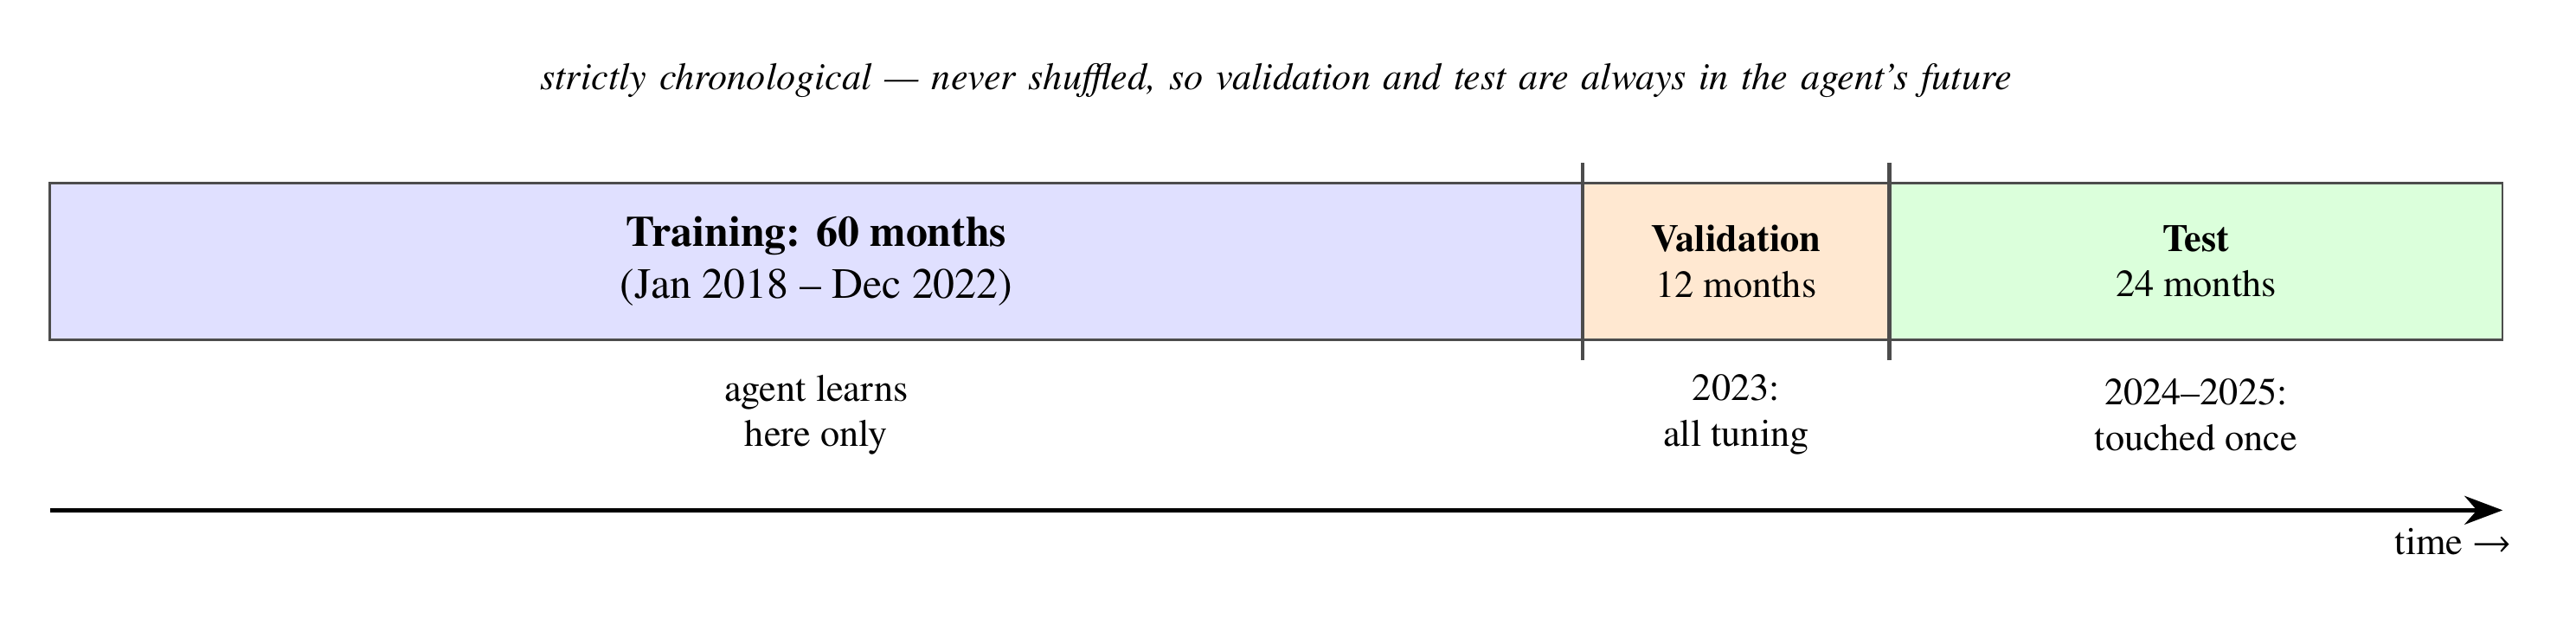
\includegraphics[width=6.29921in,height=1.51291in]{media4/media/image1.png}

\emph{Figure 4.1: Chronological split of the 96 monthly episodes: 60
training months, 12 validation months, and 24 held-out test months.}

The split is:

{\def\LTcaptype{none} % do not increment counter
\begin{longtable}[]{@{}
  >{\centering\arraybackslash}p{(\linewidth - 6\tabcolsep) * \real{0.1534}}
  >{\centering\arraybackslash}p{(\linewidth - 6\tabcolsep) * \real{0.3980}}
  >{\centering\arraybackslash}p{(\linewidth - 6\tabcolsep) * \real{0.1562}}
  >{\centering\arraybackslash}p{(\linewidth - 6\tabcolsep) * \real{0.2924}}@{}}
\toprule\noalign{}
\begin{minipage}[b]{\linewidth}\centering
\textbf{Dataset}
\end{minipage} & \begin{minipage}[b]{\linewidth}\centering
\textbf{Period}
\end{minipage} & \begin{minipage}[b]{\linewidth}\centering
\textbf{Episodes}
\end{minipage} & \begin{minipage}[b]{\linewidth}\centering
\textbf{Purpose}
\end{minipage} \\
\midrule\noalign{}
\endhead
\bottomrule\noalign{}
\endlastfoot
Training & January 2018 -- December 2022 & 60 & Learning model
parameters \\
Validation & January 2023 -- December 2023 & 12 & Selecting experimental
settings \\
Test & January 2024 -- December 2025 & 24 & Final evaluation \\
\textbf{Total} & \textbf{2018--2025} & \textbf{96} & \\
\end{longtable}
}

The episodes are also kept in chronological order within the splits and
are not randomly shuffled between these three periods. The training set
contains 60 monthly episodes and is used to learn the reinforcement
learning algorithm's parameters. The validation data set contains 12
months and is used to make decisions during development, such as fixed
trading amounts. The test set contains the final 24 months and is kept
separate from these decisions for only the final evaluation.

Maintaining a chronological split is important for financial data. This
prevents observations from later periods from entering the training set
and influencing the model's development. This would not reflect how a
trading strategy would be developed in practice.

The training period includes most market conditions, including the
volatility experienced in 2018, the COVID-19 market crash and recovery
in 2020, and the 2022 downtrend. The 2023 period is used for validation,
while 2024 and 2025 form the final test period.

The separation between validation and test data is especially important
for the experiments in Chapter 5. A configuration that performs well on
the validation period may therefore be selected to examine its
performance on the held-out test period. The test results are then used
to compare the learned strategies.

The processed episodes and their metadata are cached locally so that the
same dataset can be used consistently across all experiments.

\textbf{4.3 Training, Validation and Testing Procedure}

The experiments use a fixed sequence that separates training,
validation, and test periods. This separation ensures that the test data
are not used when making decisions about the model or experimental
setup.

\textbf{4.3.1 Training}

During training, each learning algorithm interacts with the monthly
episodes in the training period. Each algorithm is given the same market
data, state representation, portfolio conditions, and trading
constraints. The main difference between the algorithms is how they use
the collected experience to update their parameters.

REINFORCE updates the policy using the reward-to-go calculated from
completed monthly episodes. DQN updates its Q-network using transitions
sampled from the replay buffer. PPO collects fixed-length rollouts and
uses the resulting batches for several optimisation epochs.

Each configuration is trained using six random seeds. Using multiple
seeds reduces the dependence on using one particular network
initialisation or a sequence of sampled experiences and allows the
variation between runs to be reported.

The trained model from each seed is saved with its configuration so that
it can be evaluated later using the same settings.

\textbf{4.3.2 Validation}

The validation set contains the 12 monthly episodes from 2023.

This period is used for decisions that need to be made before the final
test. For example, it determines the fixed transaction amount traded for
each Buy or Sell action.

The different calibrations of transaction sizes include:

\[0.05,\ 0.10,\ 0.25,\ 0.50\]

of the initial capital.

The selection is based on the maximum portfolio exposure that can be
achieved from each action rather than on trading performance during the
test period. This prevents the action from being chosen simply because
it happens to perform well on the final evaluation data.

Once the required configuration decisions have been made, the selected
settings are fixed for testing.

\textbf{4.3.3 Testing}

The final evaluation uses the held-out data from January 2024 to
December 2025.

The test data are not used to make configuration decisions. This ensures
that results provide an independent assessment of the methods.

Each trained model is evaluated in the same trading environment and
using the same evaluation procedure, which includes the initial capital,
transaction costs, action constraints, and monthly episode structure.

For the learned agents, actions are selected intentionally by choosing
the highest-probability action for the policy-based methods or the
highest-valued action for DQN.

The portfolio outcomes are then recorded for each monthly test episode
and each random seed. This produces a consistent set of results that can
be used to compare the different learning algorithms.

The stored results therefore contain sufficient information to compare
algorithms, state representations, reward functions, and benchmark
strategies, which are presented in Chapter 5.

\textbf{4.4 Experiment Configuration}

The implementation was designed so that different experiments could be
run by changing their settings without changing the overall trading
environment or learning algorithm settings.

For this reason, experiments are defined through configuration files or
parameters rather than by manually changing the source code for each
run. Each experiment is therefore linked to a specific configuration
that records the conditions used to produce it.

This separates experiment settings from the environment's implementation
and learning algorithms, allowing the same code to run different state,
reward, and action configurations.

\textbf{4.4.1 Configuration Parameters}

The configuration records the main settings that can affect an
experiment\textquotesingle s outcome. These include:

\begin{itemize}
\item
  learning algorithm;
\item
  state representation and state dimensionality;
\item
  reward formulation;
\item
  transaction fee;
\item
  fixed transaction amounts;
\item
  risk-penalty coefficient, where applicable;
\item
  action model;
\item
  random seed;
\item
  training settings;
\item
  evaluation settings.
\end{itemize}

Using this approach reduces the need to manually change the source code
between experiments. It also makes the experimental process easier to
track, since each result can be linked directly to the configuration
that produced it.

This is particularly important for the experiments reported in Chapter
5, where several state, reward, and action configurations are compared.

\textbf{4.4.2 Algorithm Configuration}

The experiment uses the same starting capital and transaction cost
across all three learning algorithms. The initial capital is set to

\[C_{0} = \$ 10,000\]

and a transaction fee of 0.05\% is applied to each trade opened.

The main settings used for REINFORCE, DQN, and PPO are shown below.

{\def\LTcaptype{none} % do not increment counter
\begin{longtable}[]{@{}
  >{\centering\arraybackslash}p{(\linewidth - 6\tabcolsep) * \real{0.1885}}
  >{\centering\arraybackslash}p{(\linewidth - 6\tabcolsep) * \real{0.2837}}
  >{\centering\arraybackslash}p{(\linewidth - 6\tabcolsep) * \real{0.2699}}
  >{\centering\arraybackslash}p{(\linewidth - 6\tabcolsep) * \real{0.2501}}@{}}
\toprule\noalign{}
\begin{minipage}[b]{\linewidth}\centering
\textbf{Parameter}
\end{minipage} & \begin{minipage}[b]{\linewidth}\centering
\textbf{REINFORCE}
\end{minipage} & \begin{minipage}[b]{\linewidth}\centering
\textbf{DQN}
\end{minipage} & \begin{minipage}[b]{\linewidth}\centering
\textbf{PPO}
\end{minipage} \\
\midrule\noalign{}
\endhead
\bottomrule\noalign{}
\endlastfoot
Network & MLP with 2 hidden layers of 128

\(d \rightarrow 128 \rightarrow 128 \rightarrow 3\) & MLP with 2 hidden
layers of 128

\(d \rightarrow 128 \rightarrow 128 \rightarrow 3\) & \(MlpPolicy\)

\(d \rightarrow 128 \rightarrow 128\) \\
Activation & tanh & ReLU & \\
Optimiser & Adam & Adam & Adam \\
Learning rate & \(10^{- 3}\) & \(10^{- 3}\) & \({3*10}^{- 4}\) \\
Discount factor \(\gamma\) & 0.99 & 0.99 & 0.99 \\
Replay buffer & --- & 50,000 & --- \\
Batch size & Episode & 64 & 64 \\
Target network update & --- & Every 500 steps & --- \\
Exploration & Policy sampling & \(\epsilon - greedy\) & Policy
sampling \\
\(\epsilon\ schedule\) & --- & 1.0 → 0.05 & --- \\
PPO clipping & --- & --- & 0.2 \\
GAE & --- & --- & 0.95 \\
PPO epochs & --- & --- & 10 \\
Entropy coefficient & --- & --- & 0 \\
Training budget & 80,000 steps & 80,000 steps & 80,000 steps \\
Random seeds & 42--47 & 42--47 & 42--47 \\
\end{longtable}
}

All three methods use the same training budget of 80,000 steps and the
same six random seeds to keep the computational budget similar
throughout when comparing performance.

The experiments consider the different state and reward configurations
described in Chapter 5. These include the standard nine-feature state,
the ten-feature state with drawdown, the primary wealth-change reward,
the risk-aware reward, and the alternate action configurations.

The implementation also treats each trading position size as a
configurable parameter. Its final value is selected using the predefined
validation procedure. Chapter 5 reports the different values and their
effect on trading results as part of the experimental findings.

\textbf{4.4.3 Benchmark Implementation}

The learned agents are evaluated against predefined benchmark
strategies. These benchmarks provide reference points for interpreting
whether the learned policies provide useful trading behaviour.

The main benchmarks include a cash-only strategy and buy-and-hold
strategies that reflect the different interpretations of the trading
environment.

For the true buy-and-hold benchmark, the available initial capital is
used to purchase the asset at the beginning of the episode. The position
is then retained until the final trading step, when it is liquidated.
The same transaction fee and terminal liquidation procedure used by the
learned agents are applied to this benchmark.

This is different from a strategy that gradually purchases the asset
using the same monetary amount as the learning agents. A gradual
accumulation strategy may not become fully invested within a short
monthly episode, particularly when the trading amount is small.

For this reason, gradual accumulation is not treated as equivalent to
conventional buy-and-hold. The latter represents a fully invested
position from the beginning of the episode and therefore provides a
clearer reference for the performance of the learned strategies.

Where possible, the benchmark strategies use the same portfolio
accounting and evaluation procedures as the learned agents. This ensures
that differences in the reported results are primarily due to the
strategies themselves rather than differences in how their portfolios
are calculated.

\textbf{4.5 Implementation Verifications}

Before using the experimental results for analysis, the implementation
was tested to ensure that it followed the definitions and constraints
established in Chapter 3.

These tests check that the environment, data pipeline, reward
calculation, and action constraints behave as intended.

The final implementation includes 21 automated tests covering all major
components, all of which pass.

\textbf{4.5.1 Environment and Portfolio Tests}

The environment tests focus on the correctness of the portfolio
calculations during trading.

The tests verify that portfolio wealth matches the cash balance and the
market value of current holdings. They also check that Buy and Sell
actions update the portfolio correctly and that transaction fees are
included in all transactions.

The tests further verify that invalid actions are handled correctly and
that each monthly episode ends without an open position.

These checks are important because an error in portfolio accounting
would affect the reported rewards and performance measures for all three
learning algorithms. Such an error could therefore lead to incorrect
conclusions even if the learning algorithms were implemented correctly.

\textbf{4.5.2 Feature and Data Tests}

The feature tests check that the state representation follows the
intended information structure defined in Chapter 3.

The tests verify that features do not use future information and that
rolling features access the necessary historical information when moving
from one monthly episode to the next. They also check that the state
dimensions and feature ordering match the reported configurations.

The chronological split is tested to ensure that the training,
validation, and test periods remain separate.

This testing process identified an important implementation issue. In an
earlier version of the pipeline, rolling features were recalculated
separately for each monthly episode. As a result, the rolling windows
restarted at the beginning of every month rather than continuing from
the previous observations, leading to the first set of poor results.

This caused incomplete feature windows in the first days of an episode.
In the affected implementation, this issue occurred in approximately
43.1\% of episode steps.

This caused incomplete feature windows at episode boundaries, affecting
about \textbf{43.1\% of episode steps} in that implementation.

This problem is what led to \textbf{calculating rolling market features
on the continuous dataset} \textbf{before dividing the data into monthly
episodes}. The corrected pipeline was then tested again to confirm that
the required historical information was retained across episode
boundaries.

This correction mattered because it affected not only data processing
but also how the state was presented to the learning algorithms.

\textbf{4.5.3 Reward and Risk Tests}

The reward tests verify that the primary wealth-change reward
corresponds to the change in portfolio wealth with no risk penalty
applied.

The risk-aware reward is tested separately to see whether increasing
drawdown does not lead to an increase in the reward due to the risk
penalty applied.

An additional test checks the relationship between the risk-aware reward
and the state representation. A risk-aware reward cannot be paired with
a state that does not have the drawdown feature.

The implementation uses this restriction so an inconsistent combination
of state and reward settings cannot run accidentally.

These tests therefore ensure that the relationship between state
representation and reward design described in Chapter 3 is also
maintained in the implemented system.

\textbf{4.5.4 Action-Masking Tests}

The action-masking tests verify that the environment correctly
identifies invalid actions that cannot be executed under the current
portfolio conditions.

The tests check that the Buy action is unavailable when the portfolio
has insufficient cash and that the Sell action is unavailable when the
agent does not hold enough of the asset. They also verify the different
configurable fixed trading amounts.

A defensive check is also included in the environment so that an invalid
action supplied externally is converted to Hold rather than being
executed.

Logs monitor these checks during the experiments. After the final
experiment, the recorded rate of invalid actions was zero during
evaluation, confirming that the action masks accurately prevented the
learning algorithms from executing any invalid trades during the testing
period.

\textbf{4.6 Implementation Corrections}

\textbf{4.6.1 Problems Identified During Development}

The verification process identified several implementation issues before
the final experiments were run.

The main issues involved the feature calculation, benchmark
implementation, and the risk-aware reward configuration.

First, the rolling market features using past observations did not
initially contain the needed historical context when a new monthly
episode began. These meant that some features were calculated using
shorter windows than intended.

Second, an earlier version of the buy-and-hold benchmark used the same
transaction size as the learning algorithms. This did not represent a
fully invested buy-and-hold strategy, where an asset is bought at the
beginning of an episode and held untouched till the end of the
experiment, and it caused understated exposure and benchmark
performance.

Third, the risk-aware reward could initially be used without requiring
the drawdown feature in the state. This created a mismatch between the
information needed by the reward and the information supplied to the
agent because drawdown information was unavailable.

These issues were treated as implementation errors that needed
correcting because leaving any of them in place would affect the
validity of comparisons between the learning algorithms and benchmark
strategies.

\textbf{4.6.2 Correction and Re-verification}

Each identified issue was addressed through a general correction
process:

\begin{enumerate}
\def\labelenumi{\arabic{enumi}.}
\item
  the problem was identified through testing or auditing the
  implementation;
\item
  its potential effect on the experiment results;
\item
  the relevant part of the implementation that needed correcting;
\item
  adding or updating verification tests where necessary after the
  correction;
\item
  completely running the verification tests again.
\end{enumerate}

The buy-and-hold issue, for example, shows why this process was
necessary. The affected implementation understated the benchmark by
approximately \textbf{\$38.95 per month}, or \textbf{21.6\%} before
correction.

These values describe only the incorrect implementation, which has been
discarded, and are reported here only to show the potential impact of
the error. They are not presented as findings about the
asset\textquotesingle s or the market\textquotesingle s performance.

After the corrections, the complete automated batch tests were run
again, and all 21 tests passed.

The final experiment results in Chapter 5 come only from the corrected
implementation, not the earlier incorrect versions.

\textbf{4.7 Complete Implementation Pipeline}

The complete implementation pipeline is a sequence of stages, from
collecting historical market data to storing the final evaluation test
results.

The first stage loads the SPY OHLCV data, including an initial warm-up
period needed to calculate the rolling features. The market features are
then calculated on the continuous dataset using only information
available up to said observation. Once feature construction is complete,
the data are divided chronologically into the training, validation, and
test datasets.

The observations are then grouped into monthly episodes. At the start of
each episode, the portfolio resets to the initial capital with no asset
holdings. At each timestep, the learning algorithm receives the current
state and selects one of the valid available actions. The trading
environment then executes the action with the transaction fee, updates
the portfolio, returns the reward, and moves to the next state.

REINFORCE, DQN, and PPO all interact with the same trading environment.
Their main difference is how each algorithm processes the experience to
update their model parameters.

After training and validation, the final experiment settings are fixed,
and the trained models are evaluated on the held-out 2024-2025 test
datasets. The resulting metrics, monthly results, training information,
configuration settings, and performance measures are stored together
with information about the software environment used to produce them.

The overall implementation can therefore be summarised as:

\textbf{Market data → warm-up period → feature calculation →
chronological split → monthly episodes → trading environment →
experimental configuration → learning algorithm → training → validation
→ fixed configuration → held-out testing → stored results}

This pipeline clearly links the methodological decisions defined in
Chapter 3, their implementation in the system, and the experiment
results presented in Chapter 5.

Figure 4.2 summarises the flow.

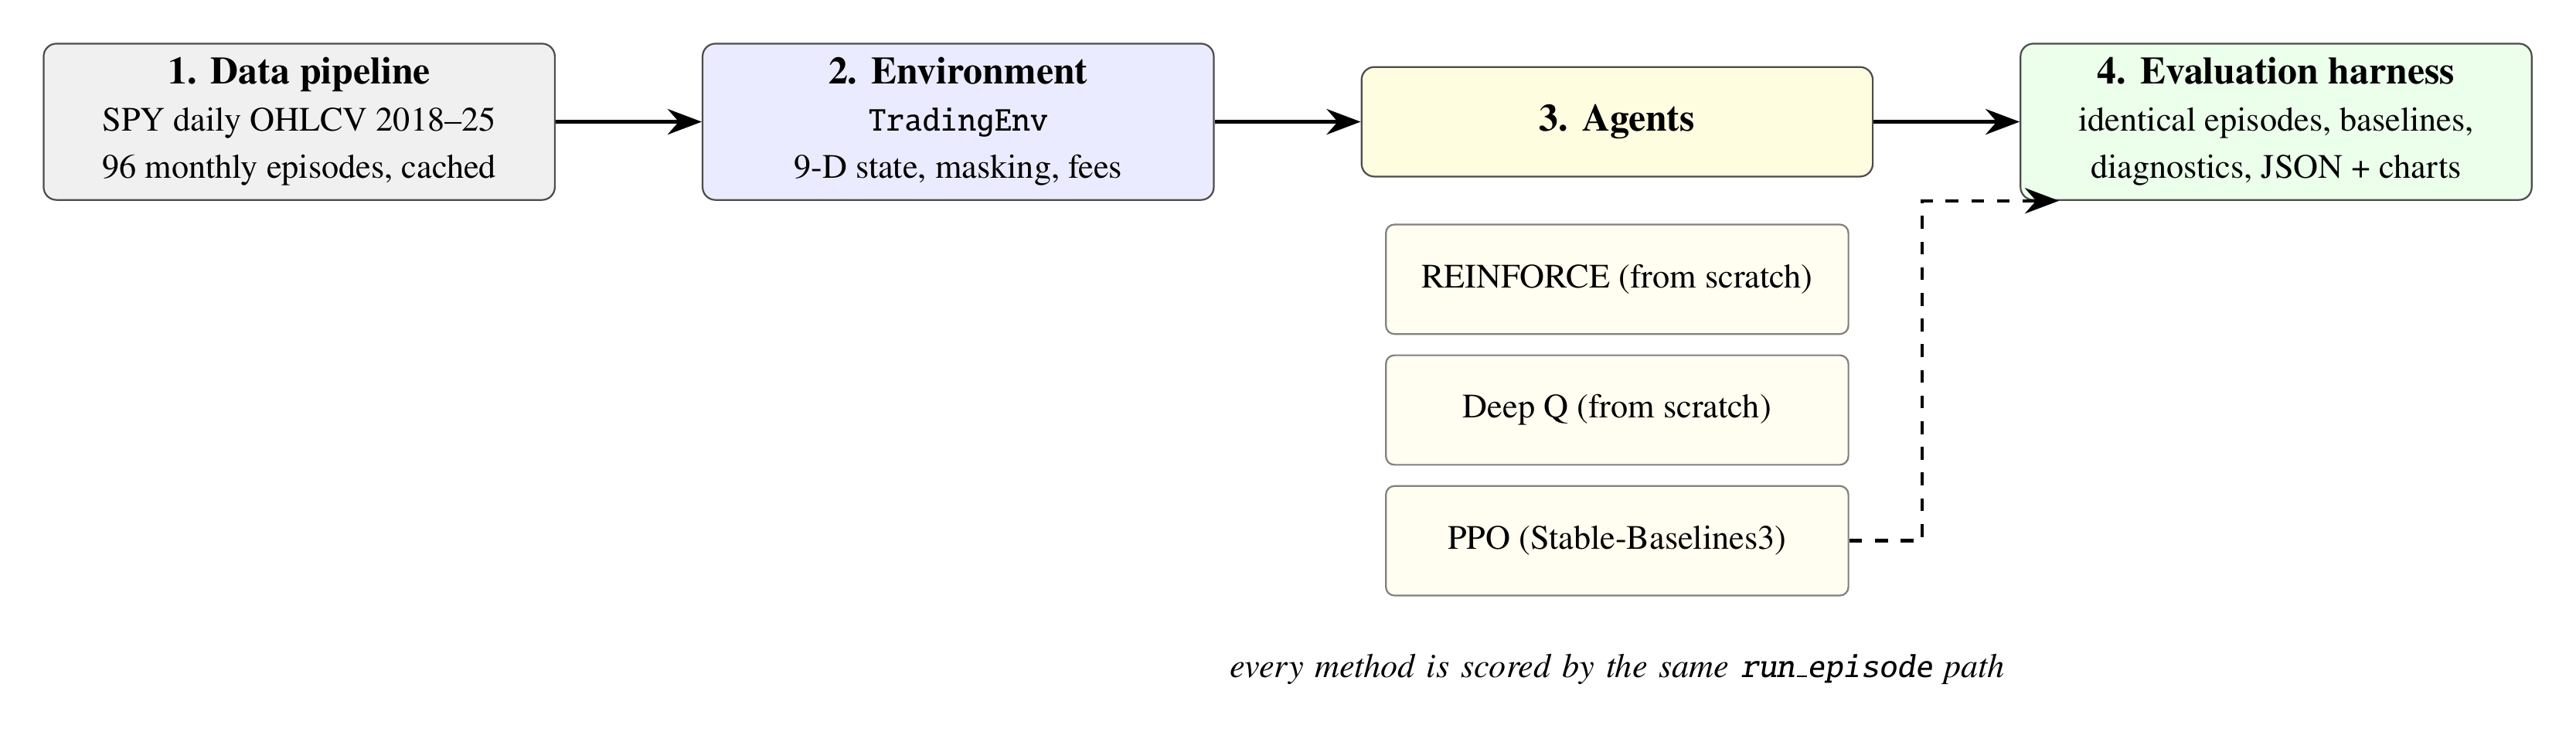
\includegraphics[width=6.29921in,height=1.81435in]{media4/media/image2.png}

\emph{Figure 4.2: System architecture showing the data flow described in
Section 4.7. All learned algorithms and benchmark strategies are
evaluated using the same episode runner, ensuring that the comparison
uses the same evaluation procedure\textbf{.}}

\textbf{Chapter 5}

\textbf{Experimental Results and Analysis}

\textbf{5.1 Introduction}

This chapter reports and analyses the experiment results from the
trading environment and learning algorithms described in Chapter 4. The
experiments examine the financial performance of the learned agents, the
effects of two state representations, and their respective reward
functions.

The experiments are structured around four questions that directly
relate to the objectives of the dissertation to increase portfolio
wealth:

\begin{enumerate}
\def\labelenumi{\arabic{enumi}.}
\item
  \textbf{Performance:} Do the learned agents outperform appropriate
  simple benchmarks on unseen data after accounting for transaction
  costs?
\item
  \textbf{Behaviour:} Do the learned agents make use of the market and
  portfolio information provided in the state representations?
\item
  \textbf{State representation:} Does adding the drawdown feature to the
  main nine-feature state affect the learned behaviour or financial
  performance?
\item
  \textbf{Reward:} Does the risk-aware reward improve the balance
  between return and drawdown, rather than simply encouraging the agent
  to trade less?
\end{enumerate}

A key part of the analysis is determining whether the learned strategies
outperform simple strategies. Buy-and-hold, for example, is an important
benchmark here. A learned agent producing a positive return does not
necessarily indicate that it has learned a useful trading strategy if a
simple investment strategy achieves a similar or better result.

For this reason, the analysis considers both \textbf{financial
performance} and \textbf{agent behaviour}. Financial performance is
evaluated using measures including wealth change, exposure, trading
activity, drawdown, and Sharpe ratio. Behavioural analysis examines
whether an agent\textquotesingle s actions change as the state changes.
This helps to identify a policy that responds to state information
rather than one that follows a fixed trading pattern.

\textbf{5.2 Experiment Protocols and Evaluation Criteria}

5.2.3 Experimental configurations

5.2.4 Evaluation metrics

5.2.5 Benchmark strategies

\textbf{5.3 Fixed Trade Size Tuning}

Before comparing the learned agents with the benchmarks, the fixed
transaction size used by the learning agents must be finalized.
Determining this trading-action size matters because the amount traded
at each decision point determines how quickly the agent can build or
reduce its position during a monthly episode.

In the trading environment, each Buy or Sell action changes the trade by
a fixed fraction of the initial capital. A smaller value gives the agent
finer control over its position but also means that more trading
decisions are needed to reach a high level of asset exposure. A larger
value lets the agent build its position more quickly but provides less
control over the size of each change.

This creates a problem between the learned agents and the buy-and-hold
benchmark. Buy-and-hold invests the available capital at the beginning
of the episode, while a trading agent must build its position through
repeated actions. If the trade size uses a small, fixed transaction
size, the agent will need several trading days to reach a similar
exposure as buy-and-hold and may not overall reach the same exposure
within a typical month. Poor results could therefore arise from the
fixed trade amounts rather than from the learned policy.

The trade size was therefore calibrated using the validation data to
select the most stable size before running the main comparison between
learning algorithms on the held-out data.

\textbf{5.3.1 Exposure available under different transaction sizes}

The validation experiment measures the maximum exposure reachable during
a month using a policy that always buys whenever the action is
available, for each fixed transaction size. The validation set contains
12 monthly episodes, with an average length of approximately 20.8
trading days. Table 5.1 and Figure 5.1 show the results.

\emph{Table 5.1: Attainable exposure for each fixed trade amount on the
validation months. The policy buys whenever a purchase is valid.}

{\def\LTcaptype{none} % do not increment counter
\begin{longtable}[]{@{}
  >{\centering\arraybackslash}p{(\linewidth - 6\tabcolsep) * \real{0.1725}}
  >{\centering\arraybackslash}p{(\linewidth - 6\tabcolsep) * \real{0.3929}}
  >{\centering\arraybackslash}p{(\linewidth - 6\tabcolsep) * \real{0.2374}}
  >{\centering\arraybackslash}p{(\linewidth - 6\tabcolsep) * \real{0.1973}}@{}}
\toprule\noalign{}
\begin{minipage}[b]{\linewidth}\centering
\textbf{Trade amount}
\end{minipage} & \begin{minipage}[b]{\linewidth}\centering
\textbf{Buys Days required to purchase a full asset}
\end{minipage} & \begin{minipage}[b]{\linewidth}\centering
\textbf{Mean maximum exposure}
\end{minipage} & \begin{minipage}[b]{\linewidth}\centering
\textbf{Mean wealth change}
\end{minipage} \\
\midrule\noalign{}
\endhead
\bottomrule\noalign{}
\endlastfoot
0.05C₀ & 20 & 0.450 & +\$95.49 \\
0.10C₀ & 10 & 0.690 & +\$121.79 \\
0.25C₀ & 4 & 0.838 & +\$167.39 \\
0.50C₀ & 2 & 0.886 & +\$162.77 \\
Buy-and-hold & --- & 0.910 & +\$166.92 \\
\end{longtable}
}

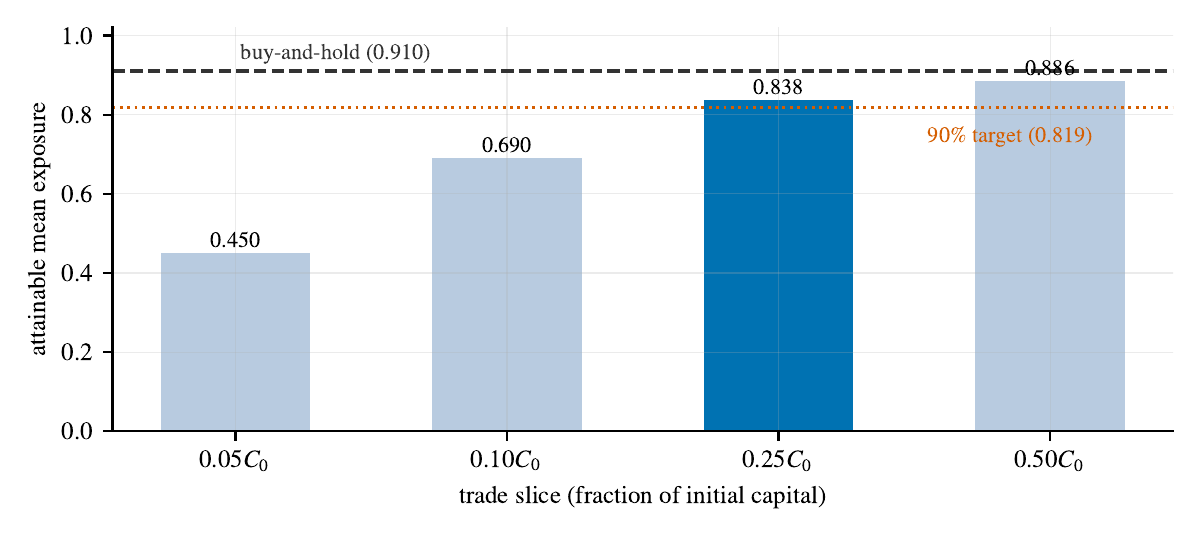
\includegraphics[width=5.8in,height=2.61in]{media4/media/image3.png}

\emph{Figure 5.1: Exposure ceilings from Table 5.1. The 0.25 C₀ trade
amount (highlighted) is the smallest that clears the 90\% target of
buy-and-hold's exposure; the 0.10 C₀ amount cannot reach it even in
principle.}

The results show that the original\(\ 0.10C₀\) trade size restricts the
agent\textquotesingle s asset exposure. This trade size requires ten buy
days to fully invest in that asset, but the average episode is only 20.8
trading days long, so half a typical month passes before full investment
is even possible.~ Its mean maximum exposure is 0.690, which is also
significantly below the 0.910 asset exposure for the simple buy-and-hold
strategy.

Hence, even a policy that buys whenever possible cannot reach the same
level of exposure as a simple benchmark during a typical monthly
episode. This matters when analysing the agent's performance. A low
return may result from poor decision-making, but it may also result from
the trading size preventing the agent from investing enough in the
asset. The two outcomes should be treated distinctly.

The \(\ 0.25C₀\) trade size was therefore selected as the primary
configuration, reaching 0.838 exposure, which corresponds to
approximately 92\% of the buy-and-hold exposure. This selection was
based on the criteria that exposure must reach at least 90\% of the
buy-and-hold, since no trade size can reach that level completely.

The buy-and-hold exposure of 0.910 gives an average exposure of
approximately 0.819 under this criterion. The \(0.25C₀\) trade size
therefore satisfies the requirement as the smallest tested trade size
whose exposure is close to the benchmark.

Increasing the trade size setting to \(0.50C₀\) raises exposure
slightly, from 0.838 to 0.886, but makes each individual action much
larger, giving the agent less control over gradual exposure changes.

Based on this calibration, the \(0.25C₀\) size balances maximum asset
exposure and control over position changes. It gives the learned agents
a reasonable opportunity to reach the benchmark level without using a
much coarser \(0.50C₀\) trade size.

\textbf{5.4 Do the Learned Policies Use Their Observations?}

The Financial performance of the portfolio trading agent on its own does
not show whether a learned agent is actually using the information
contained in its state representation. For example, an agent that buys
whenever buying is possible can perform well in a rising market without
using any of the market information its state provides.

This requires examining the behavioural patterns of the agents' learned
strategies to identify whether a policy selects a different action when
the state changes, provided the available valid actions remain the same.
This shows that the policy responds to its observed state rather than
simply following action constraints and can be classified as
\textbf{state-dependent.}

The experiment is performed on the validation data using the calibrated
\(0.25C₀\) trade size decided in Section 5.3, with the nine-feature
state and the primary wealth-change reward. This test aims only to
analyse behavioural differences between the algorithms by determining
whether changes in the information provided to the agent are reflected
in its decisions. It is not used to determine the final financial
performance of the agents.

Every cell was trained from scratch for this study: six seeds per
method, 80,000 steps each.

\textbf{5.4.1 Behaviour of the learned policies}

\emph{Table 5.2: Behavioural Results on the validation months (0.25 C₀
trade size, nine-feature state, wealth-change reward, six freshly
trained seeds). The always-buy strategy shows the maximum asset exposure
this trade size can reach.}

{\def\LTcaptype{none} % do not increment counter
\begin{longtable}[]{@{}
  >{\raggedright\arraybackslash}p{(\linewidth - 10\tabcolsep) * \real{0.1676}}
  >{\centering\arraybackslash}p{(\linewidth - 10\tabcolsep) * \real{0.1665}}
  >{\centering\arraybackslash}p{(\linewidth - 10\tabcolsep) * \real{0.1664}}
  >{\centering\arraybackslash}p{(\linewidth - 10\tabcolsep) * \real{0.1666}}
  >{\centering\arraybackslash}p{(\linewidth - 10\tabcolsep) * \real{0.1663}}
  >{\centering\arraybackslash}p{(\linewidth - 10\tabcolsep) * \real{0.1667}}@{}}
\toprule\noalign{}
\begin{minipage}[b]{\linewidth}\centering
\textbf{Policy}
\end{minipage} & \begin{minipage}[b]{\linewidth}\centering
\textbf{Mean ΔW}
\end{minipage} & \begin{minipage}[b]{\linewidth}\centering
\textbf{Seed spread}
\end{minipage} & \begin{minipage}[b]{\linewidth}\centering
\textbf{Exposure}
\end{minipage} & \begin{minipage}[b]{\linewidth}\centering
\textbf{Trades}
\end{minipage} & \begin{minipage}[b]{\linewidth}\centering
\textbf{State-dependent}
\end{minipage} \\
\midrule\noalign{}
\endhead
\bottomrule\noalign{}
\endlastfoot
\textbf{Always-buy} & +\$167.39 & --- & 0.838 & --- & --- \\
\textbf{REINFORCE} & +\$154.96 & \$37.29 & 0.807 & 10.3 & 0/6 \\
\textbf{Deep Q-learning} & +\$86.16 & \$64.20 & 0.325 & 8.5 & 6/6 \\
\textbf{PPO} & +\$118.55 & \$167.39 & 0.596 & 3.7 & 0/6 \\
\end{longtable}
}

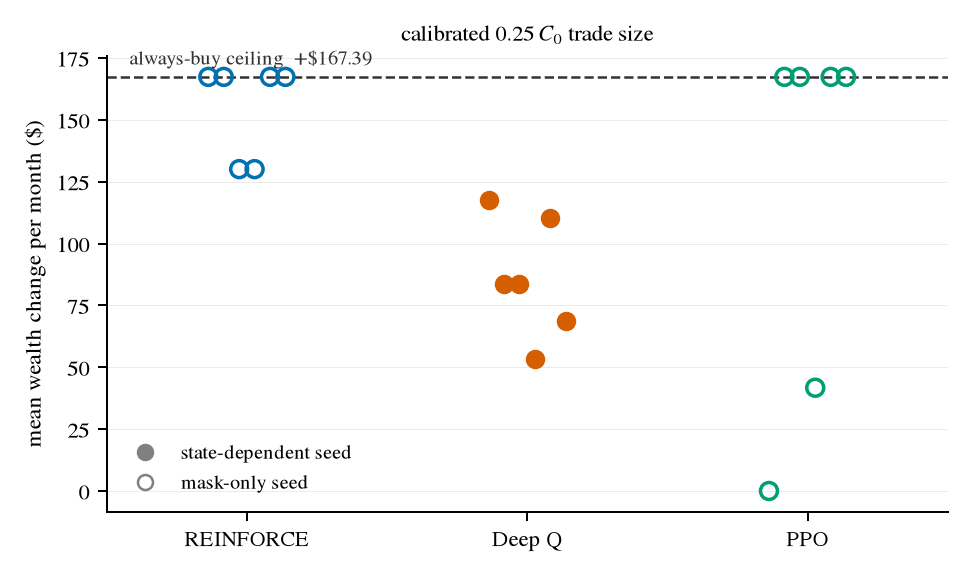
\includegraphics[width=5.8in,height=3.43704in]{media4/media/image4.png}

\emph{Figure 5.2: Results for each seed from Table 5.2. Hollow-marker
seeds show actions that don't depend on their state information;
filled-marker seeds are state-dependent ones. Policy-gradient methods
(REINFORCE, PPO) produce policies that cluster to either high exposure
or collapse towards zero, while all six Deep Q-learning seeds fall
between those corners.}

Table 5.2 summarises the outcome and Figure 5.2 shows every seed
individually. The columns read as follows. Mean ΔW is the average wealth
change per month, calculated over the 12 validation months and then over
the six seeds. Seed spread is the difference between the best and worst
seeds; a spread larger than the mean produced noticeably different
results and did not agree on a strategy. State-dependent counts how many
of the six seeds act according to the experimental behaviour being
analysed.

The REINFORCE results are clearer when the individual seeds are read.
Four of its six seeds finished at exactly +\$167.39 with an exposure of
0.838. This matches the always-buy strategy, which was set as the upper
limit. These policies buy on the first four days when buying is valid,
hold the position, and close at the end of the month. The other two
seeds earned +\$130.10 while trading 20.8 times per month: Their actions
followed a fixed pattern of trading on each bar rather than changing in
response to the market state.

PPO produced three different behaviours across its six seeds. Four seeds
reached the always-buy result of +\$167.39. One seed never traded at
all, producing a wealth change of \$0.00 and an exposure of 0.000. The
remaining seed earned +\$41.73, relying on only two trading styles. This
produced a seed spread of \$167.39, showing the large difference between
the strongest and weakest PPO runs.

Deep Q-learning is the only method where none of its seeds reached
either extreme behaviours, unlike the policy-gradient methods. Its
results ranged from +\$53.23 to +\$117.43, with a mean wealth change of
+\$86.16 and an average exposure of 0.325, less than half the 0.838
standard exposure of the always-buy strategy.

\textbf{5.4.2 State-dependence analysis}

The final column in Table 5.2 summarises the state-dependence test, with
the count representing the difference in behaviour across the six seeds

For REINFORCE, the result of 0/6 means that none of the six
independently trained policies changed their action when the state
changed while the same actions remained valid. The four seeds that
reached the maximum exposure followed the same basic rule of buying
whenever possible, while the other two followed a fixed trading pattern.
The diagnostic therefore found no evidence that these policies used
market and portfolio features to change their decisions.

Deep Q-learning produced the opposite result. All six seeds were
classified as state-dependent. Each seed selected different actions in
states where the same valid actions were available. This indicates that
the observed current state influences the decisions made by the DQN
policies.

PPO produced the same result as REINFORCE, with 0/6 state-dependent
seeds. Taken together, the splits are categorical by algorithm family
across the three methods: all six DQN seeds were state-dependent,
compared with none of the 12 policy-gradient seeds from REINFORCE and
PPO.

\textbf{5.4.3 Interpretation of the learned trading behaviour}

The different results across the three methods suggest that the learning
approach had a strong influence on the type of trading behaviour that
developed. REINFORCE and PPO frequently moved towards simple policies
that did not change their actions in response to the observed state,
whereas Deep Q-learning showed state-dependent behaviour across all six
seeds.

One possible explanation is the difference between policy-gradient and
value-based learning. REINFORCE updates the probability of an action
according to the return that follows it. When the market generally
favours holding an asset, repeatedly buying can produce a strong return
without needing to sample other policies. The learning signal may
therefore settle on a simple high-exposure strategy for higher rewards
rather than exploring.

PPO uses a different update rule from REINFORCE, but it still learns a
policy directly. Its clipped objective prevents large policy changes,
which can make learning more stable, but it does not need the policy to
become state-dependent. If a simple trading rule produces consistently
positive returns, the policy may face little pressure to learn a more
complex relationship between state and action. The extreme seed outcomes
are what hint at this. Seeds from both policy-gradient methods finish at
the always-buy upper limit, since that is the most rewarding.

Deep Q-learning learns differently. Rather than adjusting action
probabilities directly, it estimates the value of each available action
in the current state and picks the action with the highest estimate at
each step. When future estimated values differ, the chosen action
changes accordingly, and the agent has to distinguish between these
actions. The state-dependent behaviour therefore becomes a structural
property of this algorithm rather than an achievement, as it necessarily
depends on the changes in the market and portfolio state.

These explanations should be treated as interpretations of observed
behaviours rather than as direct evidence of the internal learning
process. This experiment was not designed to find out the precise reason
the algorithms moved to these different strategies. They are, however,
consistent, as different seeds show that learning algorithms affect how
available state information is used to develop a trading strategy.

\textbf{5.5 Effect of the State Representation}

Chapter 3 defines the nine-feature state as the main state
representation used in this study. It includes market, portfolio,
position, and time information. Drawdown is intentionally treated
separately as an additional risk-related feature rather than as the last
stage of the state design.

This experiment therefore focuses on a specific question: does adding
drawdown to the nine-feature state produce a meaningful change in
performance or behaviour when the reward function remains unchanged?

The comparison keeps the following conditions fixed:

\begin{itemize}
\item
  The same wealth-change reward;
\item
  the same \(0.25C₀\) trade size;
\item
  the same held-out test period;
\item
  the same six random seeds.
\end{itemize}

The intended difference between the two configurations is therefore only
the inclusion of drawdown in the state.

\textbf{5.5.1 Nine-Feature vs Ten-Feature State}

{\def\LTcaptype{none} % do not increment counter
\begin{longtable}[]{@{}
  >{\raggedright\arraybackslash}p{(\linewidth - 16\tabcolsep) * \real{0.1541}}
  >{\centering\arraybackslash}p{(\linewidth - 16\tabcolsep) * \real{0.1241}}
  >{\centering\arraybackslash}p{(\linewidth - 16\tabcolsep) * \real{0.1018}}
  >{\centering\arraybackslash}p{(\linewidth - 16\tabcolsep) * \real{0.0952}}
  >{\centering\arraybackslash}p{(\linewidth - 16\tabcolsep) * \real{0.1213}}
  >{\centering\arraybackslash}p{(\linewidth - 16\tabcolsep) * \real{0.0890}}
  >{\centering\arraybackslash}p{(\linewidth - 16\tabcolsep) * \real{0.0876}}
  >{\centering\arraybackslash}p{(\linewidth - 16\tabcolsep) * \real{0.0952}}
  >{\centering\arraybackslash}p{(\linewidth - 16\tabcolsep) * \real{0.1318}}@{}}
\toprule\noalign{}
\begin{minipage}[b]{\linewidth}\centering
\textbf{Method}
\end{minipage} & \begin{minipage}[b]{\linewidth}\centering
\textbf{State}
\end{minipage} & \begin{minipage}[b]{\linewidth}\centering
\textbf{ΔW (\$)}
\end{minipage} & \begin{minipage}[b]{\linewidth}\centering
\textbf{Spread}
\end{minipage} & \begin{minipage}[b]{\linewidth}\centering
\textbf{Exposure}
\end{minipage} & \begin{minipage}[b]{\linewidth}\centering
\textbf{Trades}
\end{minipage} & \begin{minipage}[b]{\linewidth}\centering
\textbf{DD}
\end{minipage} & \begin{minipage}[b]{\linewidth}\centering
\textbf{Sharpe}
\end{minipage} & \begin{minipage}[b]{\linewidth}\centering
\textbf{State-dep.}
\end{minipage} \\
\midrule\noalign{}
\endhead
\bottomrule\noalign{}
\endlastfoot
\textbf{REINFORCE} & 9-feature & +171.51 & 24.7 & 0.810 & 10.3 & 0.0266
& 0.675 & 0/6 \\
\textbf{REINFORCE} & 10-feature & +167.39 & 24.7 & 0.794 & 13.0 & 0.0263
& 0.670 & 0/6 \\
\textbf{Deep Q} & 9-feature & +74.68 & 71.4 & 0.312 & 8.2 & 0.0124 &
0.507 & 6/6 \\
\textbf{Deep Q} & 10-feature & +77.81 & 89.5 & 0.354 & 7.4 & 0.0140 &
0.505 & 6/6 \\
\textbf{PPO} & 9-feature & +127.35 & 179.8 & 0.598 & 3.7 & 0.0195 &
0.562 & 0/6 \\
\textbf{PPO} & 10-feature & +159.97 & 94.0 & 0.759 & 7.3 & 0.0250 &
0.671 & 1/6 \\
\end{longtable}
}

\emph{Table 5.3: Results of the nine- and ten-feature states on the test
data (wealth-change reward, 0.25 C₀ trade size, six seeds). DD shows the
mean drawdown within each episode, while State-dep. shows the number of
seeds where actions changed with the observed state.}

The effect of adding drawdown and the changes in mean wealth performance
for REINFORCE and DQN are small.

For REINFORCE, wealth change falls from \$171.5 with the nine-feature
state to +\$167.39 with the ten-feature state. The difference is only
−\$4.12 per month against a seed spread of \$24.70 for both
configurations, which is considerably larger than the mean wealth
change.

The behavioural result also remains unchanged. None of the six seeds are
classified as state-dependent in either configuration. Adding drawdown
therefore did not produce a noticeable change in the behaviour of the
REINFORCE policies.

DQN shows a small change in the opposite direction. Wealth increases
from +\$74.68 to +\$77.81, a change of +\$3.13 per month. The seed
spreads are \$71.40 and \$89.50, respectively, so the change between the
two state configurations is again much smaller than the variation across
seeds.

The behavioural result is unchanged for DQN. All six seeds remain
state-dependent with both state representations.

PPO appears to improve, from +\$127.35 to +\$159.97, gaining \$32.62.
However, the result needs to be considered alongside the variation
between seeds. The nine-feature configuration has a spread of
\$179.80---larger than the mean itself --- but it narrows to \$94.00 in
the ten-feature configuration, with only one seed becoming
state-dependent.

The change in the mean is therefore not enough, on its own, to show that
adding drawdown caused the improvement.

\textbf{5.5.2 Analysis When Drawdown Was Added}

The other performance measures columns tell the same story in different
parts. For DQN, average exposure rose from 0.312 to 0.354, and mean
drawdown from 0.0124 to 0.0140 after adding that feature to the state
--- return, exposure, and risk all moved up together by similar
proportions. Its Sharpe ratio, however, changes very little, from 0.507
to 0.505.

The patterns noticed here suggest the additional drawdown feature did
not lead to more effective risk-aware decisions, but to slightly larger
asset exposure

The changes for REINFORCE barely move. Exposure falls from 0.810 to
0.794, while drawdown decreases slightly from 0.0266 to 0.0263, as
expected of a policy algorithm that does not read the state it is given.

The small changes in the financial measures therefore do not indicate a
change in the basic policy behaviour.

Overall, the results do not show a consistent improvement in either
performance or behaviour from adding drawdown to the state while using
the default wealth-change reward.

\textbf{5.5.3 Interpretation}

These results do not mean that drawdown information is unimportant. They
show that, in this environment, without changing the reward objective,
the additional information did not provide a clear advantage--- an agent
maximising wealth change in general rising markets has little use for
its own loss history.

This matters because Chapter 3 introduced drawdown to provide
information that could support risk-sensitive decisions. However, this
feature becomes relevant only when the agent's learning objective makes
larger drawdowns costly while increasing portfolio wealth, which is
precisely what the risk-aware reward experiment in Section 5.7 tests.

\textbf{5.6 Held-Out Test Results}

The main performance question of how each learned strategy, in its final
configuration, compares with the simple benchmarks on unseen data is
evaluated on the 24 held-out months from January 2024 to December 2025.

At this point, the main configuration has been fixed:

\begin{itemize}
\item
  nine-feature state;
\item
  wealth-change reward;
\item
  \(0.25C₀\) trade size;
\item
  0.05\% transaction fee;
\item
  six random seeds.
\end{itemize}

\textbf{5.6.1 Overall Comparison with the Benchmark Strategies}

{\def\LTcaptype{none} % do not increment counter
\begin{longtable}[]{@{}
  >{\raggedright\arraybackslash}p{(\linewidth - 14\tabcolsep) * \real{0.1676}}
  >{\centering\arraybackslash}p{(\linewidth - 14\tabcolsep) * \real{0.1210}}
  >{\centering\arraybackslash}p{(\linewidth - 14\tabcolsep) * \real{0.1177}}
  >{\centering\arraybackslash}p{(\linewidth - 14\tabcolsep) * \real{0.1364}}
  >{\centering\arraybackslash}p{(\linewidth - 14\tabcolsep) * \real{0.1146}}
  >{\centering\arraybackslash}p{(\linewidth - 14\tabcolsep) * \real{0.1139}}
  >{\centering\arraybackslash}p{(\linewidth - 14\tabcolsep) * \real{0.1177}}
  >{\centering\arraybackslash}p{(\linewidth - 14\tabcolsep) * \real{0.1111}}@{}}
\toprule\noalign{}
\begin{minipage}[b]{\linewidth}\centering
\textbf{Policy}
\end{minipage} & \begin{minipage}[b]{\linewidth}\centering
\textbf{ΔW (\$)}
\end{minipage} & \begin{minipage}[b]{\linewidth}\centering
\textbf{Spread}
\end{minipage} & \begin{minipage}[b]{\linewidth}\centering
\textbf{Exposure}
\end{minipage} & \begin{minipage}[b]{\linewidth}\centering
\textbf{Trades}
\end{minipage} & \begin{minipage}[b]{\linewidth}\centering
\textbf{DD}
\end{minipage} & \begin{minipage}[b]{\linewidth}\centering
\textbf{Sharpe}
\end{minipage} & \begin{minipage}[b]{\linewidth}\centering
\textbf{State-dep.}
\end{minipage} \\
\midrule\noalign{}
\endhead
\bottomrule\noalign{}
\endlastfoot
\textbf{Buy-and-hold} & +180.25 & --- & 0.913 & 2.0 & 0.0310 & 0.638 &
--- \\
\textbf{Always-buy (}\(\mathbf{0.25}\mathbf{C₀}\)\textbf{)} & +179.75 &
--- & 0.841 & 5.0 & 0.0274 & 0.684 & --- \\
\textbf{REINFORCE} & +171.51 & 24.7 & 0.810 & 10.3 & 0.0266 & 0.675 &
0/6 \\
\textbf{Deep Q-learning} & +74.68 & 71.4 & 0.312 & 8.2 & 0.0124 & 0.507
& 6/6 \\
\textbf{PPO} & +127.35 & 179.8 & 0.598 & 3.7 & 0.0195 & 0.562 & 0/6 \\
\end{longtable}
}

\emph{Table 5.4: test results over the 24 held-out months (2024--2025):
benchmarks and the three learned agents in their final configuration,
six seeds each.}

Table 5.4 is the central result of this dissertation.

Two simple strategies are used as benchmarks. Buy-and-hold invests the
full capital on the first day and is the benchmark an investor would
actually compare against. Always-buy at \(0.25C₀\) buys an asset at a
quarter fraction of the initial capital. This takes trades with every
valid action until it has fully invested in the asset. It represents a
strategy that buys unconditionally at the fixed trade size, without
requiring observations.

The central result is straightforward: none of the three learned agents
outperformed buy-and-hold during the held-out test period.

Buy-and-hold earned +\$180.25 per month, equivalent to a 1.8025\%
increase of the initial capital per monthly episode, and no learned
agent reached this. The closest was REINFORCE at +\$171.51, which was
\$8.74 short of buy-and-hold per month; PPO earned +\$127.35 and Deep
Q-learning +\$74.68.

Always buying at \(0.25C₀\) earned +\$179.75, within \$0.50 of
buy-and-hold, and it sets the standard a learned agent must reach/beat
before it can claim any skill, as matching it needs no market
information at all --- only buying whenever buying is available.

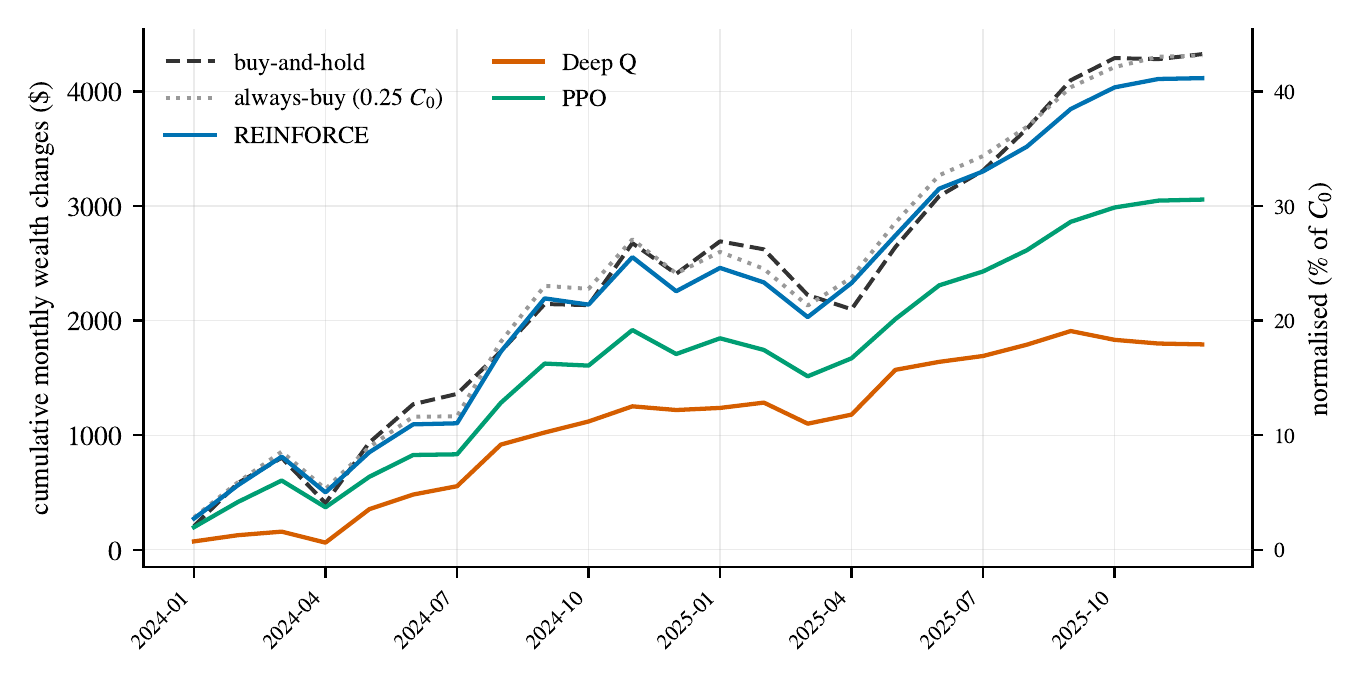
\includegraphics[width=6in,height=3in]{media4/media/image5.png}

\emph{Figure 5.3: Cumulative sum of average monthly wealth changes
across the test months. Each monthly episode resets to C₀, so the lines
show the sum of monthly gains and losses rather than compound; the right
axis expresses percentages of initial capital C₀. REINFORCE follows
Always-buy (0.25 C₀) and buy-and-hold almost exactly, while Deep
Q-learning shows a flatter line due to low exposure, including through
the March--April 2025 decline.}

Over the full two years, the gap compounds visibly in Figure 5.3:
buy-and-hold accumulates to +\$4,326 in monthly wealth change at the end
of 2025, REINFORCE to +\$4,116 closely following buy-and-hold, PPO to
+\$3,056, and Deep Q-learning at the lowest value of +\$1,792.

\textbf{5.6.2 Return and market exposure}

The exposure column explains most of the return column. The REINFORCE
result is particularly interesting; its return was close to buy-and-hold
at +\$171.51. Its average exposure was 0.810, compared with 0.913 for
buy-and-hold, and none of its six seeds were state-dependent, suggesting
the high return came mainly from staying invested rather than learning
when to enter or leave the market. Its behaviour was therefore closer to
the Always-buy at \(0.25C\) accumulation strategy. Hence why it sits
within a few percent of Always-buy results (+\$179.75, exposure 0.841).

DQN produced a different result. All six seeds were state-dependent,
showing that the agent changed its actions in response to state
information, and chose to participate the least, with the lowest
exposure of 0.312 and a wealth change of \$74.68. These results are
roughly a third of the buy-and-hold benchmarks, so the lower return may
therefore be correlated with reduced market participation.

PPO produced a return between REINFORCE and DQN, with an average wealth
change of \$127.35 and exposure of 0.598. However, its seed spread was
179.8, which is larger than its mean return. This shows that the six PPO
runs produced different outcomes and should not be treated as a single
stable trading strategy.

\textbf{5.6.3 Risk and risk-adjusted performance}

Lower returns can still be desirable if they follow a sufficient
reduction in risk. For this reason, drawdown and Sharpe ratio are also
used alongside return. Figure 5.4 puts every learned configuration in
this chapter on that scale.

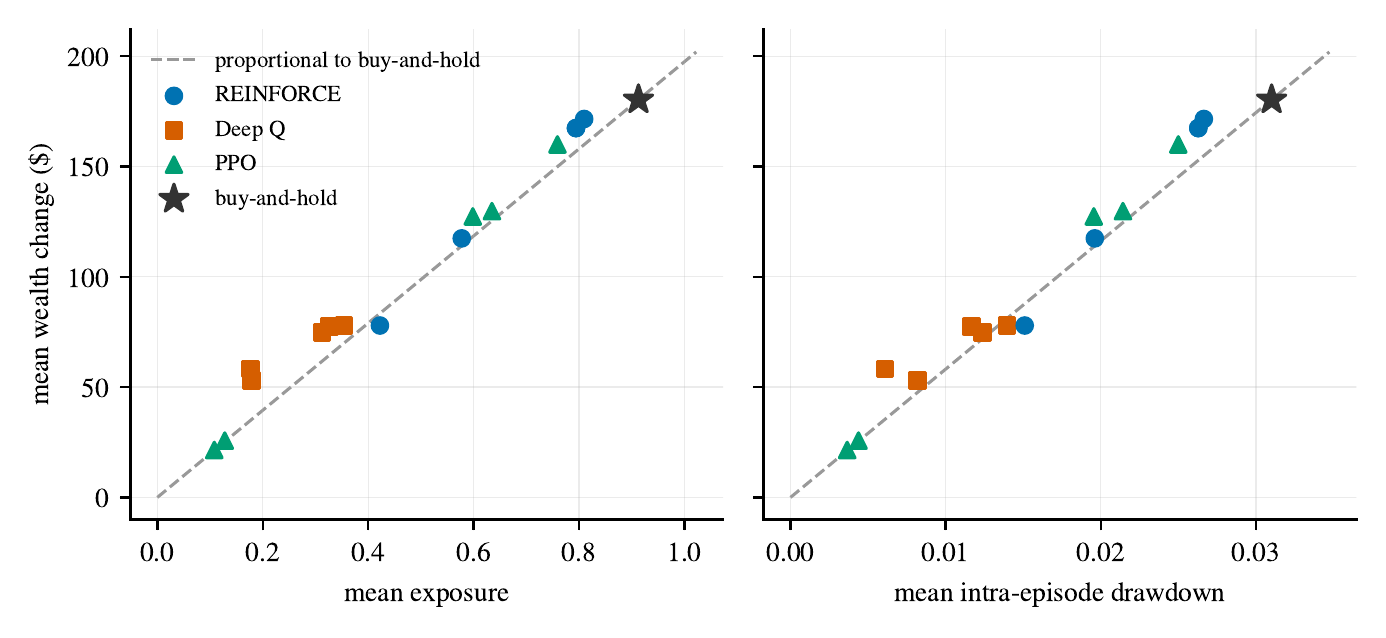
\includegraphics[width=6in,height=2.76191in]{media4/media/image6.png}

\emph{Figure 5.4: Average wealth change compared with exposure (left)
and daily drawdown (right) for every learned configuration in this
chapter. The dashed lines show the proportional relationship with
buy-and-hold. None of the learned configurations show a clear
improvement over either line.}

Buy-and-hold earned \$197 per unit of exposure. An agent that merely
holds less of the same asset lands on the dashed proportional line;
genuine downside management would appear above it.

Deep Q-learning is an informative case. It earned 41.4\% of the
buy-and-hold benchmark's return at 34.2\% of its exposure (0.312) and
40.0\% of its drawdown (0.0124) --- return and risk fell equally, which
is more like scaling down. Its Sharpe ratio of 0.507 versus
buy-and-hold's 0.638 confirms it earned less return per unit of risk
exposed to, not more.

The results therefore do not indicate that DQN achieved better
risk-adjusted performance than the benchmark. Its lower drawdown largely
came from lower exposure, not from a strategy that intentionally avoided
the market\textquotesingle s decline periods.

\textbf{5.6.4 Behaviour During the March 2025 Decline}

March 2025 provides a useful example because it was the worst test month
for the buy-and-hold benchmark. During this month, buy-and-hold lost
\$398.41, i.e. 3.9841\% of the initial capital, with a drawdown of
approximately 5.6\%. If the state-dependent agent, Deep Q-learning, had
recognised the conditions, this would have been the month to step aside.
Instead, DQN had a mean exposure of 0.490 in March--- higher than its
overall average exposure of 0.312 for the entire test period--- and lost
\$184.04, 46\% of the benchmark's loss.

These results are important when interpreting the state-dependence
finding. Even in a month when reducing exposure before the decline could
have helped, it did not significantly reduce exposure, and these March
2025 losses match its equivalent market participation. Hence, its lower
drawdown cannot be attributed to knowing when to avoid bad market
periods, but to holding less overall.

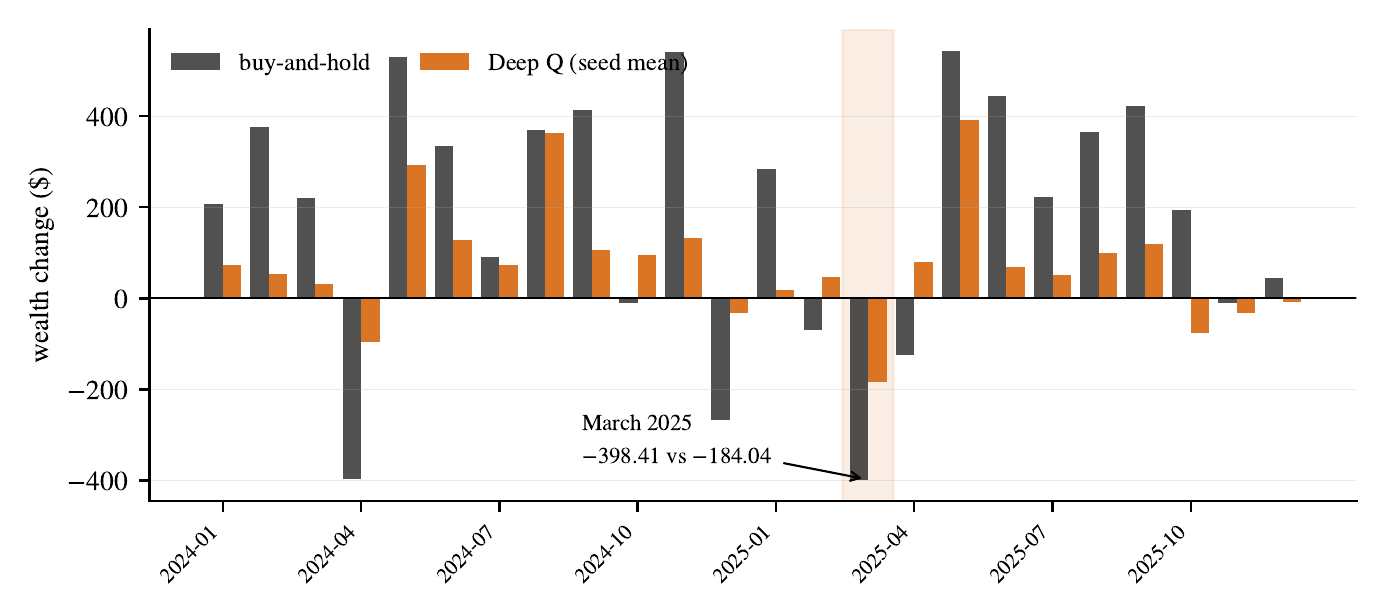
\includegraphics[width=6in,height=2.66667in]{media4/media/image7.png}

\emph{Figure 5.5: Monthly wealth changes of buy-and-hold and Deep
Q-learning over the 24 test months. The agent's bars match a 1/3 scaling
of the benchmark's bars in almost every month: In March 2025, the worst
month, it lost \$184.04 compared to the benchmark's \$398.41 loss.}

Figure 5.5 extends to all 24 months. Each pair of bars is one test
month: the dark bar represents buy-and-hold's wealth change, and the
orange bar represents the Deep Q-learning for the same month. The two
series appear to rise and fall together --- the agent's best month is
the benchmark's best month (May 2025, +\$390.80 compared to +\$543.11)
and its worst is the benchmark's worst (the discussed March 2025).

Buy-and-hold lost money in seven of the 24 months, and the agent ended
positive in three of those seven. Those three months, however, produced
little profit compared to the benchmark losses

In the two heavy down months, April 2024 (−\$396.08) and March 2025
(−\$398.41), the agent was also at a loss---approximately 24\% and 46\%
of the benchmark's loss, respectively---correlating to its 34\% average
market participation and one-third scaling to the benchmark. Where
drawdown management mattered most, the agent still left the position
open to losses.

\textbf{5.6.4 Trading behaviour and Seed consistency.}

The results also show considerable differences in consistency between
the algorithms. To examine this, we analyse seed spreads, which measure
differences between runs.

REINFORCE had the smallest seed spread (\$24.70), showing seeds agree
with each other. However, this consistency should be interpreted with
its behavioural results. All six seeds were classified as
state-independent and exhibited similar behaviour, precisely because
they agree on ignoring market information and generally being highly
exposed, as that is more rewarding. The small spread therefore does not
necessarily indicate that REINFORCE learned a more reliable trading
strategy.

DQN had a larger spread of \$71.40. This is consistent with the six
seeds learning different state-dependent policies, resulting in greater
variations in their returns.

PPO had the largest spread of \$179.80, which was greater than the mean
return, also showing that individual seeds ranged from near-inactivity
to near-full investment in Fig. 5.2, and none were state-dependent.

These results show why evaluating a single random seed would not provide
enough evidence for a reliable conclusion about the learning algorithms.
Behaviour and performance can vary considerably from one training run to
the next.
